% This appendix is bound in the supplement, not the thesis: it is the full
% treatment of the selection-channel anomaly that the thesis's discussion
% chapter reports only in summary, together with a pointer here in words
% (the thesis and this file are separate documents, so a \ref to a label
% defined in one cannot resolve in the other). No citation appears below;
% the citation-bearing sentences about this anomaly stay in the thesis
% chapter, which carries the bibliography this file does not.
\chapter{The Selection-Channel Anomaly: Full Treatment}
\label{app:anomaly}

This appendix gives the full quantitative record behind the anomaly the
thesis's discussion chapter reports in summary: an unexplained pattern in
how a pool-level demographic-parity audit drifts across a swept upstream
selection channel, observed on simulated populations kept separate from the
clinical pipeline, and reported here rather than suppressed because it does
not fit any account offered for it. Nothing in this appendix is claimed as a
contribution; it is the record a reader checking the chapter's summary of
the pattern would need.

On one simulated population, with baseline disparity held fixed, two
upstream selection channels were swept and the pool-level demographic parity
gap audited at each step. Under the first the signed gap runs from
$-0.13556$ to $-0.19435$; under the second, from $-0.11807$ to $-0.04101$.
Neither series changes sign, but the fitted drift slopes have opposite sign,
and neither series is monotone in channel strength, so the endpoints do not
describe the trajectory. Fitted as drift slopes, the two channels produce
signed drifts of opposite sign, $-0.00780$ under the first regime and
$+0.01177$ under the second. A third selection experiment on a different
pool gives a gap running from $+0.00841$ to $+0.18939$, again without a sign
change.

That third experiment was also swept across operating points, and
Figure~\ref{fig:appE-threshold-surface} shows what the sweep returned. The
audited gap is not a property of the system on its own. It moves with the
operating point and with the strength of the upstream selection, so any
single audited number describes one cell of that surface rather than the
system that produced it, and the operating point actually used crosses the
tolerance contour partway along the sweep. Over a large part of the surface
the audit also stops being able to answer at all: where the minimum
detectable gap exceeds the tolerance the audit was written against, a cell
that reads as passing is reporting a sample size rather than a system, and
the two cases are not distinguishable from the recorded pass alone.

\begin{figure}[!ht]

% Caption stays after the graphic in source order: main_supplement.tex's
% \captionsetup[figure]{position=bottom} only sets caption skip amounts, it
% does not reorder the box, so this is what actually puts the caption below
% the figure, matching main_msu.tex's figure convention (author's decision
% of 2026-08-13, recorded there) that the rest of this document follows.
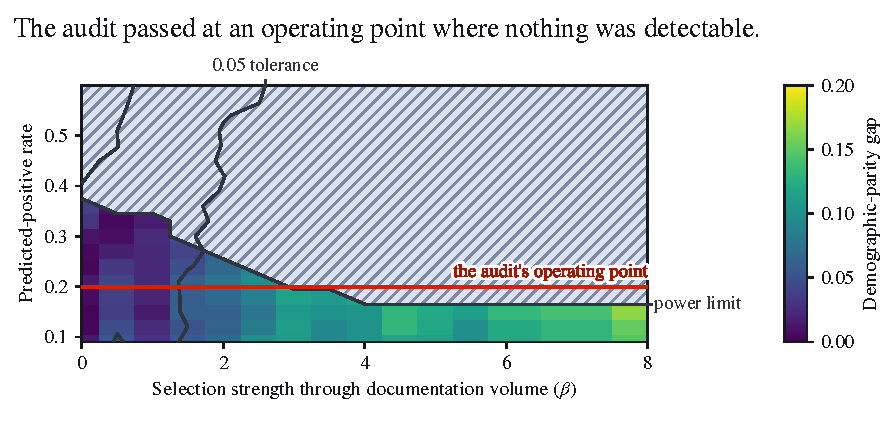
\includegraphics[width=0.98\linewidth]{figures/fig-threshold-surface.pdf}
\caption[Audited parity gap across operating points]{The audited
demographic-parity gap across operating points and selection strengths for
one selection experiment. The solid contour is the tolerance the audit was
written against. The hatched region is where the minimum detectable gap
exceeds that tolerance.}
\label{fig:appE-threshold-surface}
\end{figure}

The behaviour does not survive a controlled sweep of the same construct. A
simulator sweep over baselines, channel strengths and replicates inverts the
mapping between channel and drift direction; the grid's dimensions are not
registered, so none is quoted here. The direction in which a pool audit
drifts is therefore not a stable function of the selection channel that
produced the pool, at least across the region examined.

Five mechanism claims were proposed during this project to account for this.
Each was written down, each was tested against a parameter sweep, and each
failed; the record of those attempts is kept with the thesis's own
correction record, bound as an appendix to the thesis itself rather than
here. A sixth is not offered, and that restraint is a position rather than
an omission. The cheapest move available here is to build a story fitting
the two regimes actually observed. It would be unfalsified, because it would
be assembled after the fact from the data it purports to explain, and in the
write-up it would be indistinguishable from the five that already failed.

The supported claim is narrow and complete: on one population, with
baseline disparity fixed, the sign of the drift in a pool-level parity audit
is channel-dependent in a way a controlled sweep does not reproduce. Anyone
reading a single audited drift as evidence about an upstream selection
process is reading something whose direction was not stable where it was
checked. No subgroup harm is demonstrated, none is demonstrated anywhere in
this work, and these populations are simulated. No boundary for the effect
is claimed either, because the sweep that inverts the mapping is one
simulator with one functional form.
